\part{Mandelbrot}

\begin{figure}
    \begin{center}
        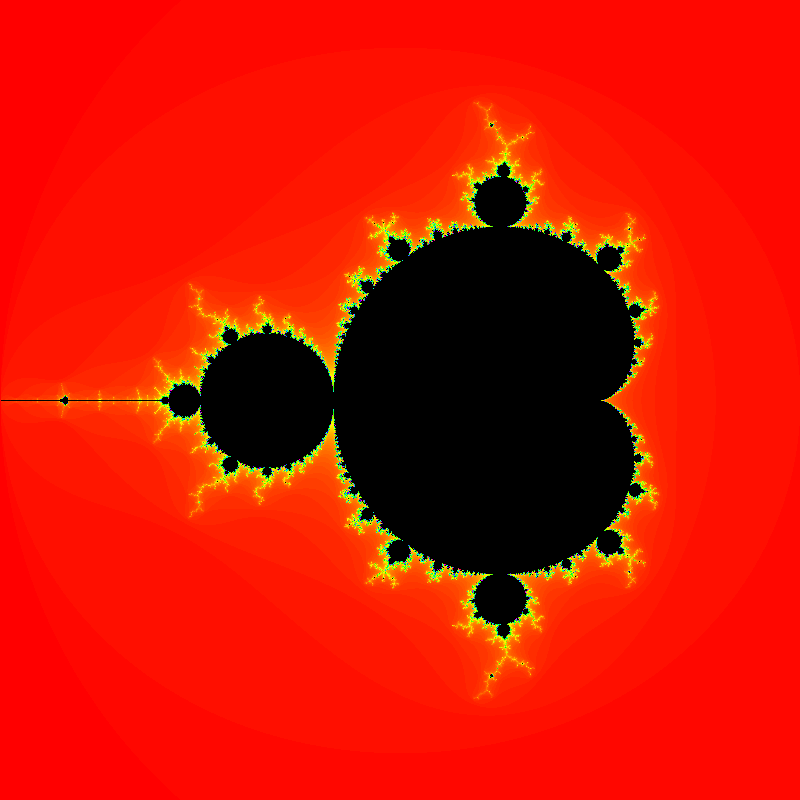
\includegraphics[width=0.6\textwidth]{mandelbrot.png}
    \end{center}
    \caption{The Mandelbrot set fractal.}
    \label{fig:mandelbrot}
\end{figure}

In this part, you will use the CImg library (\url{http://cimg.eu/}) to write a program to generate and display the \emph{Mandelbrot set} fractal; see Figure~\ref{fig:mandelbrot}.
This fractal colours each pixel of the image according to an iterated mathematical formula, as described below.

\section{} \label{core-c-first}

To generate an interesting fractal, the on-screen $x$ and $y$ coordinates must first be rescaled.
In the skeleton project the pixel coordinates range from $0$ to $800$,
whereas the Mandelbrot set fractal is most interesting in the region $-2 \leq x \leq 1$ and $-1.5 \leq y \leq 1.5$.

Let $p_x$ be the $x$ coordinate of the pixel. This can be remapped into the range $x_{\text{min}}$ to $x_{\text{max}}$ using the following formula:
\begin{equation*}
    x_0 = \frac{p_x}{\text{image.width}} \times \left( x_{\text{max}} - x_{\text{min}} \right) + x_{\text{min}}
\end{equation*}
The $y$ coordinate can be remapped using a similar formula.

\textbf{Implement} the above calculations for the $x$ and $y$ coordinates, at the indicated parts of \texttt{PartC\_Mandelbrot.cpp}.

\section{} \label{core-c-last}

The Mandelbrot set is based on the following sequence of numbers. Let $x_0$ and $y_0$ be the coordinates of a point in the image.
Then the sequence $x_1, y_1, x_2, y_2, x_3, y_3, \dots$ is defined\footnote{%
    If you are familiar with complex numbers, you may notice that this is equivalent to $z_{j+1} = z_j^2 + z_0$, where $z_j = x_j + y_j i$.
} recursively for $i = 0, 1, 2, 3, \dots$ by:

\begin{align*}
    x_{i+1} &= (x_i)^2 - (y_i)^2 + x_0 \\
    y_{i+1} &= (2 \times x_i \times y_i) + y_0 \\
\end{align*}

The points are coloured according to the \emph{smallest} value of $i$ for which $(x_i)^2 + (y_i)^2 \geq 4$.
If such a value of $i$ is not found after a large number of iterations (for example $i=200$), the pixel is coloured black.

\textbf{Implement} an algorithm which performs the above computation, determining the smallest value of $i$
for which $(x_i)^2 + (y_i)^2 \geq 4$ and selecting the appropriate pixel colour.
Implement the algorithm in \texttt{PartC\_Mandelbrot.cpp} so that the program generates the Mandelbrot set fractal (Figure~\ref{fig:mandelbrot}) when it is run.

\section{Stretch goal} \label{stretch-c}

Mathematicians have discovered many other fractals besides the Mandelbrot set.

\textbf{Implement} a new program, based on your Mandelbrot program,
to generate a different type of fractal which you have found online or in the academic literature.
